\let\negmedspace\undefined
\let\negthickspace\undefined
\documentclass[journal]{IEEEtran}
\usepackage[a5paper, margin=10mm, onecolumn]{geometry}
%\usepackage{lmodern} % Ensure lmodern is loaded for pdflatex
\usepackage{tfrupee} % Include tfrupee package

\setlength{\headheight}{1cm} % Set the height of the header box
\setlength{\headsep}{0mm}     % Set the distance between the header box and the top of the text

\usepackage{gvv-book}
\usepackage{gvv}
\usepackage{cite}
\usepackage{amsmath,amssymb,amsfonts,amsthm}
\usepackage{algorithmic}
\usepackage{graphicx}
\usepackage{textcomp}
\usepackage{xcolor}
\usepackage{txfonts}
\usepackage{listings}
\usepackage{enumitem}
\usepackage{mathtools}
\usepackage{gensymb}
\usepackage{comment}
\usepackage[breaklinks=true]{hyperref}
\usepackage{tkz-euclide} 
\usepackage{listings}
% \usepackage{gvv}                                        
\def\inputGnumericTable{}                                 
\usepackage[latin1]{inputenc}                                
\usepackage{color}                                            
\usepackage{array}                                            
\usepackage{longtable}                                       
\usepackage{calc}                                             
\usepackage{multirow}                                         
\usepackage{hhline}                                           
\usepackage{ifthen}                                           
\usepackage{lscape}


\renewcommand{\thefigure}{\theenumi}
\renewcommand{\thetable}{\theenumi}
\setlength{\intextsep}{10pt} % Space between text and floats


\numberwithin{equation}{enumi}
\numberwithin{figure}{enumi}
\renewcommand{\thetable}{\theenumi}


% Marks the beginning of the document
\begin{document}
\bibliographystyle{IEEEtran}
\vspace{3cm}

\title{9.4.1}
\author{EE24BTECH11030 - J.KEDARANANDA}
% \maketitle
% \newpage
% \bigskip
{\let\newpage\relax\maketitle}
\renewcommand{\thefigure}{\theenumi}
\renewcommand{\thetable}{\theenumi}
\textbf{Question}:\\\\
For each of the differential equations in Exercises 1 to 10, find the general solution:\\
$\frac{dy}{dx}=\frac{1-\cos{x}}{1+\cos{x}}$
\\\\
\textbf{Solution: }
Given differential equation:
\begin{align}
    \frac{dy}{dx} &= \frac{2 \sin^2\left(\frac{x}{2}\right)}{2 \cos^2\left(\frac{x}{2}\right)} \\
\end{align}
\begin{align}
    \frac{dy}{dx} &= \tan^2\left(\frac{x}{2}\right) \\
    \int dy &= \int \tan^2\left(\frac{x}{2}\right) dx \\
    y &= \int \sec^2\left(\frac{x}{2}\right) dx - \int 1 \, dx \\
    y &= 2 \tan\left(\frac{x}{2}\right) - x + C
\end{align}
\textbf{logic behind the iteration used in code: }\\
\textbf{Method of finite differences :}
The finite difference method is rooted in the fundamental concept of approximating derivatives using finite differences.

The derivative of $y(x)$ can be approximated as 
\begin{align}
    \frac{dy}{dx}&=\frac{y(x+h)-y(x)}{h}\\
    y(x+h)&=y(x)+h\brak{\frac{dy}{dx}}
\end{align}
Where h is a small value very close to zero.
\begin{align}
    y(x+h)=y(x)+h\brak{\frac{1-\cos{x}}{1+\cos{x}}} 
\end{align}

Let \brak{x_0,y_0} be a point on the curve.\\
Let some $x_1=x_0 +h$.Then,
\begin{align}
    y_1 = y_0+h\brak{\frac{1-\cos{x_0}}{1+\cos{x_0}}} 
\end{align}

On Generalizing the above equation, we have 
\begin{align}
    x_{n+1}&=x_{n} +h \\
    y_{n+1}&= y_{n}+h\brak{\frac{1-\cos{x_n}}{1+\cos{x_n}}}  
\end{align}

\begin{figure}[h!]
   \centering
   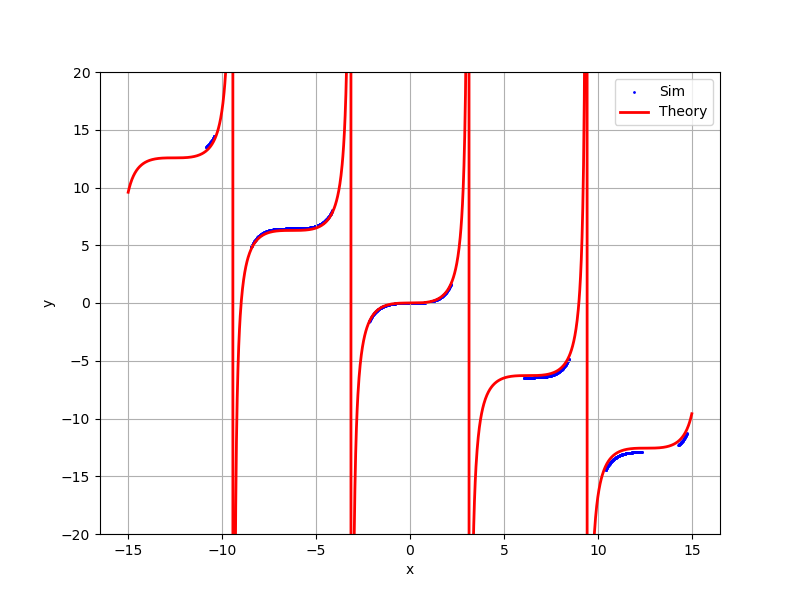
\includegraphics[width=\columnwidth]{figs/Fig1.png}
\end{figure}
\end{document}

